\chapter{実験結果}
\section{予備実験}
予備実験の結果を~(図\ref{vgg16_res},\ref{resnet_res})にそれぞれ示す.分類率は,VGG16モデルを利用したものが64.3\%,ResNetモデルを利用したものが59.5\%であった.
全般的に,データの多いクラスは精度が高い傾向にあるが,データの少ないクラスは精度が低い傾向にある.
加えて,~\(Car\)クラスは道路の進行方向に対して垂直に待機している10クラスの中で特殊なクラスであり,車などの写ったフレームの影響で分類精度が上昇していると考えられる.~\(Feed\)クラス,~\(Pet\)クラス,~\(Play\_with\_ball\)クラスは,それぞれフレーム内を人間が占める割合が多いクラスと言え,そのため混同が起こりやすいと考えられる.

%\(Look_at_Left\)クラスは


\begin{figure}[htbp]
 % \begin{tabular}{cc}
 %  \begin{minipage}{0.5\textwidth}
   \begin{center}
    
    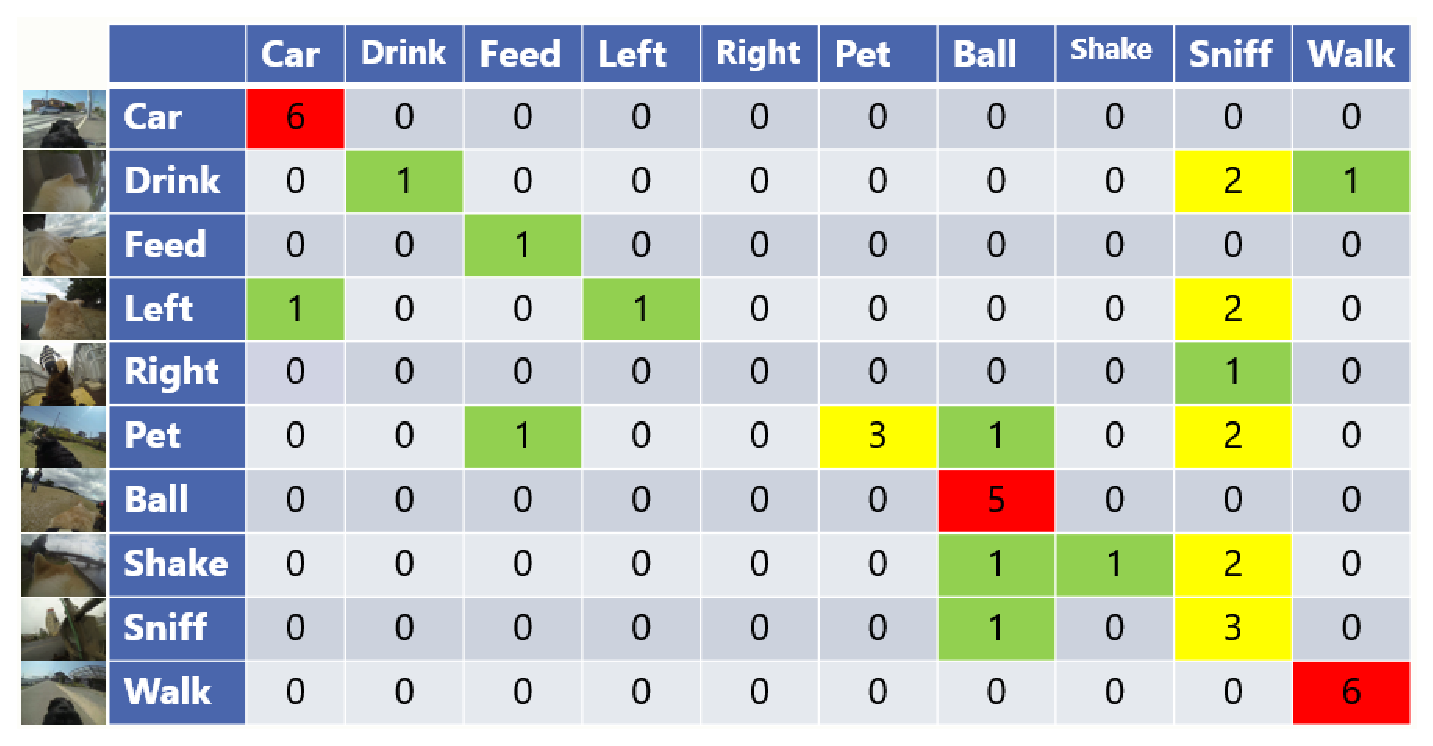
\includegraphics[scale=0.3]{./Figures/vgg16_res.eps}
    \caption{VGG16 pretrained modelによるfinetuningの結果}
    \label{vgg16_res}
   \end{center}
  % \end{minipage}
  % \begin{minipage}{0.5\textwidth}
\end{figure}
\begin{figure}[htbp]

   \begin{center}

    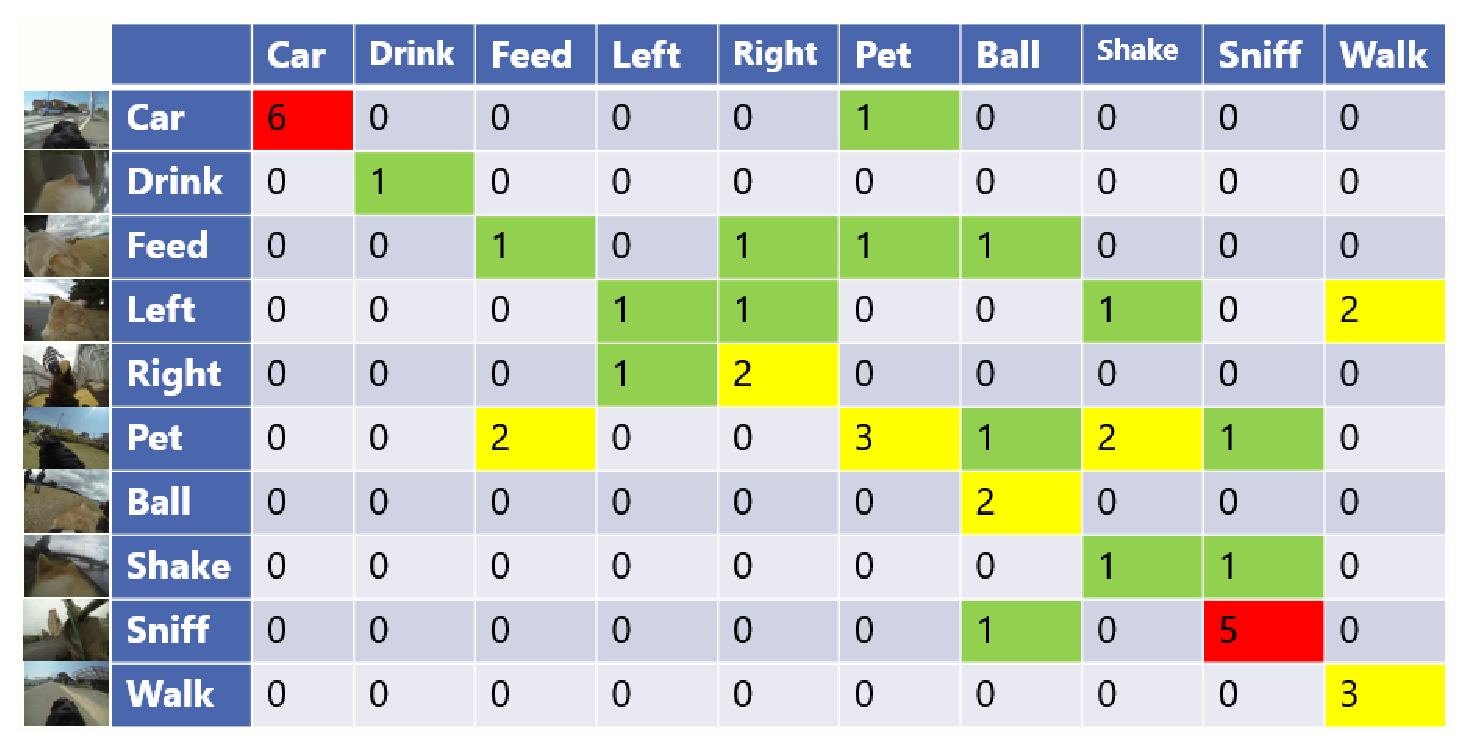
\includegraphics[scale=0.3]{./Figures/resnet_res.eps}
  \caption{ResNet pretrained modelによるfinetuningの結果}
  \label{resnet_res}
   \end{center}
 %  \end{minipage}
 % \end{tabular}
\end{figure}
\section{シングルクラス分類}
\subsection{動画像平均画像クラス認識}
\subsection{オプティカルフロー画像クラス認識}
\subsection{音声クラス認識}
\subsection{音声と動画のマルチモーダル情報クラス認識}


\section{マルチクラス認識}
\subsection{動画像平均画像クラス認識}
\subsection{オプティカルフロー画像クラス認識}
\subsection{音声クラス認識}
\subsection{音声と動画のマルチモーダル情報クラス認識}

